
% This LaTeX was auto-generated from MATLAB code.
% To make changes, update the MATLAB code and republish this document.

\documentclass{article}
\usepackage{graphicx}
\usepackage{color}

\sloppy
\definecolor{lightgray}{gray}{0.5}
\setlength{\parindent}{0pt}

\begin{document}

    
    \begin{verbatim}
clear; clc;
%H�reapparat

[x, Fs]=audioread('Reporters.mp3');
N = 1000000;


%setup frekvensakse
fd = Fs/N;
x_akse = [0:fd:Fs-fd];

x = x(1:N);

x=rot90(x);

%Foretag FFT p� signalet
X = fft(x);

y = WEIGHT_func(x,10,10,10,10,10);

%Foretag FFT p� det v�gtede signal
Y = fft(y);

%Plot de to signaler, s� man kan se forskellen i frekvenserne.
% clc;
% figure(1)
% subplot(2,1,1)
% semilogx(x_akse(1:0.5*end),20*log10(abs((2/N)*X(1:0.5*end))));
% xlabel('Frekvens')
% ylabel('dB')
% subplot(2,1,2)
% semilogx(x_akse(1:0.5*end),20*log10(abs((2/N)*Y(1:0.5*end))));
% xlabel('Frekvens')
% ylabel('dB')

soundsc(x,Fs);
pause(10);
soundsc(y,Fs);
\end{verbatim}

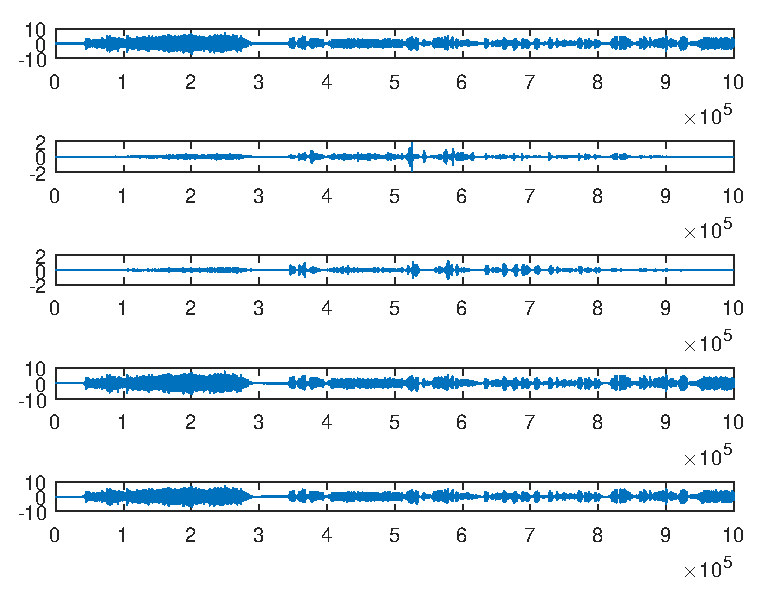
\includegraphics [width=4in]{AudioEqualizer_01.eps}



\end{document}
    
